\documentclass[10pt]{article}

%% Various useful packages and commands from different sources

\usepackage[applemac]{inputenc}
\usepackage[english]{babel}
\usepackage[T1]{fontenc}
\usepackage{cite, url,color} % Citation numbers being automatically sorted and properly "compressed/ranged".
%\usepackage{pgfplots}
\usepackage{graphics,amsfonts}
\usepackage[pdftex]{graphicx}
\usepackage[cmex10]{amsmath}
% Also, note that the amsmath package sets \interdisplaylinepenalty to 10000
% thus preventing page breaks from occurring within multiline equations. Use:
 \interdisplaylinepenalty=2500
% after loading amsmath to restore such page breaks as IEEEtran.cls normally does.

% Compact lists
\usepackage{enumitem}
\usepackage{booktabs}
\usepackage{fancyvrb}

\usepackage{listings} % for Matlab code
\definecolor{commenti}{rgb}{0.13,0.55,0.13}
\definecolor{stringhe}{rgb}{0.63,0.125,0.94}
\lstloadlanguages{Matlab}
\lstset{% general command to set parameter(s)
framexleftmargin=0mm,
frame=single,
keywordstyle = \color{blue},% blue keywords
identifierstyle =, % nothing happens
commentstyle = \color{commenti}, % comments
stringstyle = \ttfamily \color{stringhe}, % typewriter type for strings
showstringspaces = false, % no special string spaces
emph = {for, if, then, else, end},
emphstyle = \color{blue},
firstnumber = 1,
numbers =right, %  show number_line
numberstyle = \tiny, % style of number_line
stepnumber = 5, % one number_line after stepnumber
numbersep = 5pt,
language = {Matlab},
extendedchars = true,
breaklines = true,
breakautoindent = true,
breakindent = 30pt,
basicstyle=\footnotesize\ttfamily
}

\usepackage{array}
% http://www.ctan.org/tex-archive/macros/latex/required/tools/
\usepackage{mdwmath}
\usepackage{mdwtab}
%mdwtab.sty	-- A complete ground-up rewrite of LaTeX's `tabular' and  `array' environments.  Has lots of advantages over
%		   the standard version, and over the version in `array.sty'.
% *** SUBFIGURE PACKAGES ***
\usepackage[tight,footnotesize]{subfigure}
\usepackage[top=2.2cm, bottom=2.2cm, right=1.7cm,left=1.7cm]{geometry}
\usepackage{indentfirst}


%\setlength\parindent{0pt}
\linespread{1}

\usepackage{mathtools}
\DeclarePairedDelimiter{\ceil}{\lceil}{\rceil}
\DeclarePairedDelimiter{\floor}{\lfloor}{\rfloor}
\DeclareMathOperator*{\argmax}{arg\,max}
\newcommand{\M} {\mathtt{M}}
\newcommand{\dB} {\mathrm{dB}}
\newcommand{\tr} {\mathrm{tr}}



\graphicspath{ {figures/} }

% equations are numbered section by section
%\numberwithin{equation}{section}


\begin{document}
\title{Digital Transmission - Homework 3}
\author{Andrea Dittadi, Davide Magrin, Michele Polese}

\maketitle

%%%%%%%%%%%%%%%%%%%%%%%%%%%%%%%%%%%%%%%%%
%%%%%%%%%%%%%% PROBLEM 1 %%%%%%%%%%%%%%%%
%%%%%%%%%%%%%%%%%%%%%%%%%%%%%%%%%%%%%%%%%

\section*{Problem 1}

% Spiegare cosa mandiamo e come lo generiamo
In this problem the channel $q(n\frac{T}{4})$ is given at $T_c = \frac{T}{4}$. The goal is to estimate at the receiver the timing phase $t_0$ and the equivalent channel impulse response in $T$ with LS method.
The setting of the system is as in Fig.~\ref{fig:channel_T4}. In order to perform LS estimation the first $L + N_{seq} = 15 + 10$ symbols of the sequence $a_k$ are binary symbols out of a QPSK constellation with $\sigma_a^2 = 2$. 
In particular they are $1+j$ and $-1-j$ and map the $+1$ and $-1$ values of a ML sequence of length $L = 15$, partially repeated by $N_{seq}=10$. Then QPSK data follows. 
The conversion between a bit stream and QPSK is carried out by the \texttt{bitmap} function. %% TODO some more on this?? Give a better formulation

\begin{figure}
	\centering
	\includegraphics[width = 0.8\textwidth]{channel_T4}
	\caption{System setting for problem 1}
	\label{fig:channel_T4}
\end{figure}

%%TODO Does Eq go in dB???? 

% Spiegare che channel_output funziona da polifase
The noisy output $r_n$ of the channel is computed with a polyphase version of the channel impulse response $q(nT_c)$. Each branch is $q^{i}(mT) = q(mT + i)$ with $i \in [0, 3]$ , and since it is not time-varying it is possible to directly compute the convolution of each branch and the $a_k$ sequence. At the output of each convolution white noise $w_n$ is added, with variance $\sigma_w^2 = \frac{\sigma_a^2 E_q}{4 \Gamma} = -19.2411$ dB, where $\sigma_a^2 = 2$, $E_q = 2.3819$ and $\Gamma = 20$ dB is the given SNR at receiver input. Then a parallel to series converter generates the output at time $T_c$.

% !!! Spiegare come stimiamo t0, riportare l'equazione (Formula 7.269, channel_estimator)
The first operation which the receiver does is estimating $t_0$ as optimal timing phase in $T_c$. In particular, given the stream of symbols $r_n$, and the knowledge of the ML sequence $a_l, l\in [0, L-1]$, the receiver computes

\begin{equation}
	m_{opt} = \argmax_m | x_{ra}(mT_c) | = \argmax_{m} | \frac{1}{L} \sum_{l = 0}^{L - 1} x(lT + mT_c)a^* (l) |
\end{equation}
for $ 0 < m < 40$ and finds that
\begin{equation}
	m_{opt} = 10
\end{equation}
\begin{equation}
	t_{0} = m_{opt}T_c = 10 T_c
\end{equation}

% Spiegare differenza tra m_opt (in T/4, che è t0), init_offs (in T/4) e delay (in T)
% Is it really useful? Michele
Remeber that $t_0 = 10$ in $T_c$ and the corresponding $D_{ch} = (t_0 \% 4)T = 2T$ represent the number of samples after which the receiver receives the first sample of the training sequence multiplied by $h_0$, which is the coefficient of the channel impulse response with the gratest amplitude. In other words, if the receiver and the transmitter use the same time index $k$ and if $x_k$ is the output at time $T$ of the receiver then
\begin{equation}
x_{k} = h_0a_{k-D_{ch}} + i_k, \quad i_k = \sum_{\substack{i = -N_1 \\ i \neq 0}}^{N_2} h_i a_{k-D_{ch}-i}
\end{equation}
where $i_k$ is the inter-symbol interference. Therefore, if $t_0 = 10T_c$ and $D_{ch} = 2T$ there could be at most 2 precursors (i.e. the coefficients of $h_i$ for $i = -N_1, \dots, -1$), and they can be equal to 0 (they don't introduce ISI but just the delay $D_{ch}$) or different from 0 but with an amplitude lower than $h_0$. 

The receiver can now the estimate of the channel impulse response at time $T$. The output of the channel $r_n$ is sampled at $n = t_0 + kT$ to get $x_k = r_{t_0 + kT}$. Then the LS estimate is computed using the symbols of the known ML sequence $a_k$ sent and a suitable section of the output. Note that the training sequence sent of lenght $L + N_{seq} = 25$ has $N_{seq} = 10$ which is enough to avoid the transient of the channel which is $N - 1$, with $N = N_1 + N_2 + 1$ which is the real length of the impulse response.
Note also that the LS method can estimate a causal impulse response, $\tilde{h}_j, j = 0, \dots, N$, while the channel impulse response could have some precursors which are different from 0, and therefore an anticausal component. In order to correctly estimate $h_i, i = -N_1, \dots, N_2$, given a supposed length $\hat{N} = \hat{N}_1 + \hat{N}_2 + 1$, LS considers $a_k, k = 0, \dots, L+\hat{N}-1$ and the output $x_k, k = D_{ch} - N_1, \dots, D_{ch} - N_1 + L + \hat{N} - 1$ and it performs the estimation in the standard way. This is the same as considering a causal impulse response, with $\hat{N}$ coefficients, but since we suppose that $N_1$ assumes a given value in $0, D_{ch}$, then it is possible to shift the estimate left of $N_1$ samples and obtain the estimate for $\hat{h}_i, i = -N_1, N_2$. 
The actual estimation is performed as in \cite[p.~246]{bc}, i.e. using a $L \times \hat{N}$ observation matrix

\begin{equation}
	\boldsymbol{\mathcal{I}} =
 \begin{bmatrix}
  a(\hat{N}-1) & \cdots & a(0) \\
  \vdots  & \ddots & \vdots  \\
a[(\hat{N}-1)+(L-1)] & \cdots & a(L-1) \\
 \end{bmatrix}
\end{equation}
and a desired sample vector
\begin{equation}
\mathbf{o}^T = \left[ x(\hat{N}-1)\;,\; \ldots\; , \;x((\hat{N}-1)+(L-1)) \right].
\end{equation}
Therefore we can solve the LS problem as
\begin{equation}
	\hat{\mathbf{h}}= \mathbf{\Phi}^{-1} \boldsymbol{\vartheta}, \quad\mathrm{ with } \quad \mathbf{\Phi}=\boldsymbol{\mathcal{I}}^H \boldsymbol{\mathcal{I}} \quad \mathrm{ and }\quad \boldsymbol{\vartheta} = \boldsymbol{\mathcal{I}}^H \mathbf{o}.
\end{equation}

In particular, in order to estimate as first the length $\hat{N} = N_1 + N_2 + 1$ of the impulse response and $N_1, N_2$, we operate as follows. Let $N_{max} = N_{seq} = 10$ the maximum possible length $\hat{N}$ of the impulse response. As first, we set $N_1 = 0$ and compute the functional of the error 
\begin{equation} 
	\mathcal{E} = \frac{1}{L}\sum_{k = \hat{N} - 1}^{(L-1)+(\hat{N}-1)}|d(k)-\hat{d}(k)|^2
	\label{eq:functional}
\end{equation}
for $N_2 = 0, 1, \dots, N_{max} - N_1 - 1$. This procedure is repeated for $N_1 = 1$ and $2$. The functionals $\mathcal{E}$ for different $N_1$ are then plotted together, against $N_2$, in Fig.~\ref{fig:functional}.
\begin{figure}
	\centering
	\includegraphics[width = 0.8\textwidth]{error_func_p1}
	\caption{$\mathcal{E}$ vs $N_2$ for different $N_1$}
	\label{fig:functional}
\end{figure}
It can be seen that there's a knee for $N_2 = 4 \forall N_1$, therefore we pick $N_2 = 4$. Then $N_1$ that minimizes $\mathcal{E}$ should be chosen, therefore $N_1 = 2$. However the 3 curves are very close to each other, and choosing $N_1 = 0$ would bring a similar functional $\mathcal{E}$ but a much lower complexity for Viterbi and FBA in the second problem. 

In Tables~\ref{table:h0} and~\ref{table:h2} are reported the amplitude and phase of $h_i, i = -N_1, \dots, N_2$, while in Fig.~\ref{fig:hi_p1} is reported the amplitude of both the choice $N_1 = 0$ and $N_1 = 2$. Note that they are very similar.


% !!! Riportare valori di {h_i_hat} in una tabella, ampiezza e fase
\begin{table}
	\centering
	\begin{tabular}{c|c|c|c|c|c}
		$i \in [-N_1, N_2]$ & 0 & 1 & 2 & 3 & 4 \\ \hline
		$|h_i|$ 		& 0.7140  &  0.2463  &  0.1553  &  0.5778  &  0.4001 \\
		$\angle(h_i)$ 	& -2.5815  &  1.3137  & -2.5666  & -1.5096  & -1.6715 \\
	\end{tabular}
	\caption{Amplitue and phase of $h_i, i \in [-N_1, N_2]$, for the choice $N_1 = 0$}
	\label{table:h0}
\end{table}

\begin{table}
	\centering
	\begin{tabular}{c|c|c|c|c|c|c|c}
		$i \in [-N_1, N_2]$ & -2 & -1 & 0 & 1 & 2 & 3 & 4 \\ \hline
		$|h_i|$ 	&	0.0121  &  0.0137  &  0.7136   & 0.2446  &  0.1551  &  0.5853  &  0.4068 \\
		$\angle(h_i)$ &	0.3575  & -2.0494  & -2.5692   & 1.3064  & -2.5498  & -1.5017  & -1.6574 \\
	\end{tabular}
	\caption{Amplitude and phase of $h_i, i \in [-N_1, N_2]$, for the choice $N_1 = 2$}
	\label{table:h2}
\end{table}

% !!! Plottare {h_i_hat} per i = -N_1, ..., N_2
\begin{figure}
 \centering
 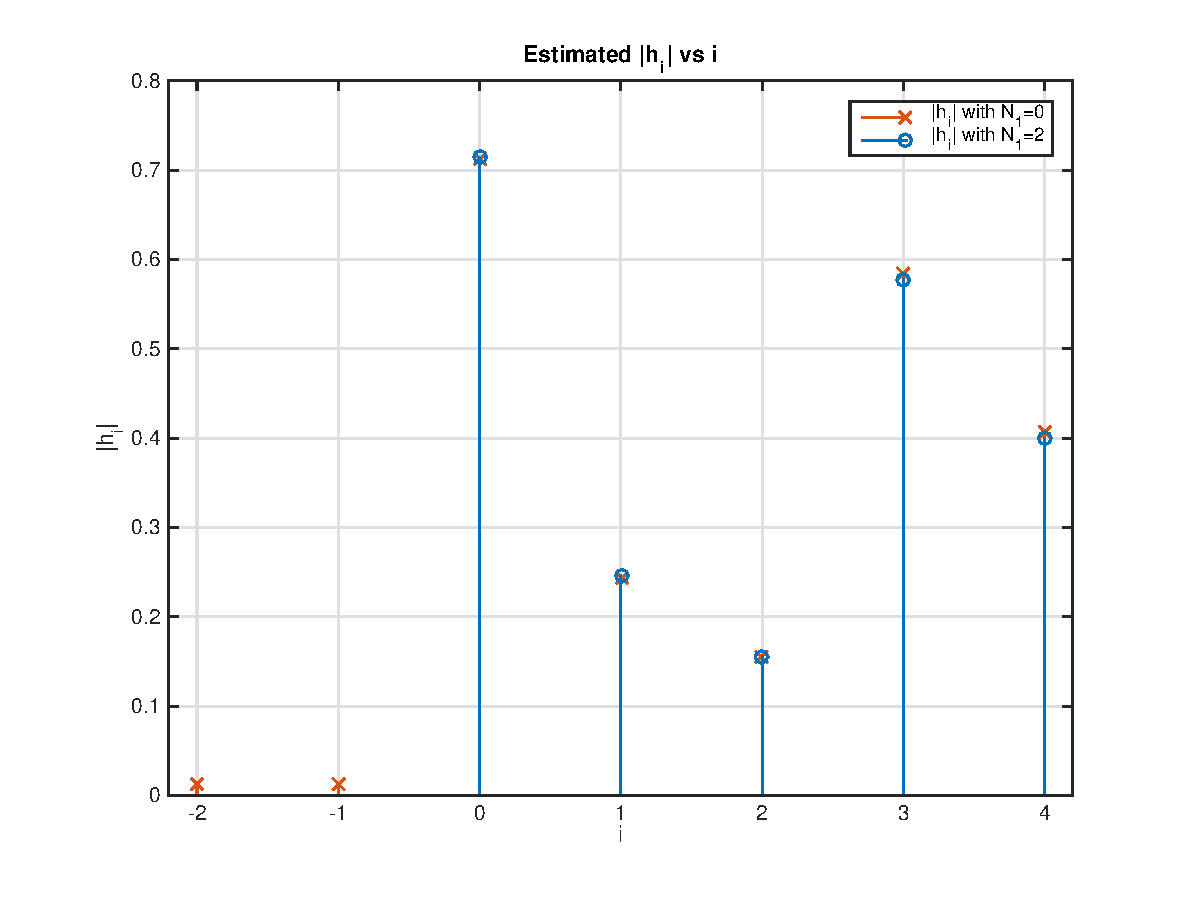
\includegraphics[width = 0.9\textwidth]{hi_p1}
 \caption{$|h_i|, i \in [-N_1, N_2]$ for $N_1 = 0$ and $N_1 = -2$}
 \label{fig:h1p1}
\end{figure}

% !!! Determinare la stima della varianza del rumore, sigma_w_hat_squared, compararla con sigma_w_squared in dB.
The noise that the channel introduces is $\sigma_w^2 = -19.2411$ dB, while the estimate $\hat{\sigma}_w^2 = something = -20.5327$ dB is lower (for the choice $N_1 = 0$, or $\hat{\sigma}_w^2 = -20.851$ for $N_1 = -2$). Note that this is the value given by a single estimate and not an expectation. However, this shows that a sequence of the given length $L = 15$ is too short to correctly estimate the real noise of the channel, since it averages on a number of noise samples which is close to the length of the impulse response we are trying to estimate. Indeed, by using a longer ML sequence (say 127) the estimate obtained is much closer to the real value also in each single realization. 

% !!! Comparare la stima di Lambda_n_hat con il valore "vero" di Lambda_n_hat, fare le considerazioni su LS per cui il Lambda_n teorico raddoppia quando si usano i simboli ±1±j al posto di ±1.
At last, some considerations on the fact that the sequence used in this problem is a binary mapping in a QPSK constellation with $\sigma_a^2 = 2$ of a PN sequence. In particular let $a_l = (1+j) p_l$ with $p_l = \pm 1$ a symbol of the PN sequence. Then the autocorrelation of the sequence, of periodicity L, is
\begin{equation}
	r_a(n) = \frac{1}{L}\sum_{l = 0}^{L-1} a_l a^*_{l-n} = \\
	\frac{1}{L}\sum_{l = 0}^{L-1} (1+j)p_l (1-j)p^*_{l-n} = 
	\frac{2}{L} \sum_{l= 0}^{L-1} p_l p^*_{l-n} = 2 r_p(n)
\end{equation}
with 
\begin{equation}
	r_p(n) = 
  	\begin{cases}
    1       & \quad \text{if } n =0 \\
    -\frac{1}{L}  & \quad \text{if } n \neq 0 \\
  \end{cases}
\end{equation}
Therefore let $\Phi(i, n) = [\mathbf{\Phi}]_{i, n}$. Then
\begin{equation}
	\Phi(i, n) = (L -1 + N - N + 1)r_a(i-n) = 2Lr_p(i-n)
\end{equation}
At the same time $\vartheta(n) = 2Lr_{dp}(n)$ with $\boldsymbol{\vartheta} = [\vartheta(0), \dots, \vartheta(N-1)]$.

\clearpage

%%%%%%%%%%%%%%%%%%%%%%%%%%%%%%%%%%%%%%%%%
%%%%%%%%%%%%%% PROBLEM 2 %%%%%%%%%%%%%%%%
%%%%%%%%%%%%%%%%%%%%%%%%%%%%%%%%%%%%%%%%%

\section*{Problem 2}

% Breve descrizione del sistema in T

% Se non fatto nel problema 1 riportare le considerazioni su N_1

% Considerazioni sull'implementazione di LE e DFE, riportare i grafici di Jmin (qualche grafico), considerazioni su M1, M2, D, riportare i grafici di \hat{h}, c, psi, b per \Gamma = 10 dB

% Considerazioni su Viterbi, Kd, grafico della distribuzione

% Considerazioni su FBA, implementazioni ecc

% Grafici del BER, sia per canale stimato che per canale vero, riportando il numero di bit per le simulazioni



\begin{thebibliography}{10}

\bibitem{bc}
Benvenuto, Cherubini, Algorithms for Communications Systems and their Applications, Wiley, 2004

\end{thebibliography}

\end{document}
